\documentclass[fleqn]{article}
\usepackage[nodisplayskipstretch]{setspace}
\usepackage{amsmath, nccmath, bm}
\usepackage{amssymb}
\usepackage{enumitem}
\usepackage{etoolbox}
\usepackage[normalem]{ulem}
\usepackage[hidelinks,colorlinks=true,urlcolor=blue,linkcolor=black]{hyperref}
\usepackage{graphicx}
\usepackage{float}
\usepackage{changepage}
\usepackage{environ,capt-of}
\usepackage{matlab-prettifier}

\let\oldfigure\figure% Store original figure float environment
\let\endoldfigure\endfigure
\RenewEnviron{figure}[1][H]{% Update figure environment
  %\par\vspace{\intextsep}% Assume in-text placement, so insert appropriate vertical spacing
  \noindent
  % \patchcmd{<cmd>}{<search>}{<replace>}{<success>}{<failure>}
  \patchcmd{\BODY}{\caption}{\captionof{figure}}{}{}% Replace \caption with \captionof{figure} inside \BODY
  % Set "figure"
  \begin{minipage}{\linewidth}
    \BODY
  \end{minipage}
  %\par\vspace{\intextsep}% Assume in-text placement, so insert appropriate vertical spacing
}

\makeatletter
\begingroup
  \catcode`\$=6 %
  \catcode`\#=12 %
  \gdef\href@split$1#$2#$3\\$4{%
    \hyper@@link{$1}{$2}{\uline{$4}}% or \underline
    \endgroup
  }%
\endgroup

\newcommand{\zerodisplayskip}{
	\setlength{\abovedisplayskip}{0pt}%
	\setlength{\belowdisplayskip}{0pt}%
	\setlength{\abovedisplayshortskip}{0pt}%
	\setlength{\belowdisplayshortskip}{0pt}%
	\setlength{\mathindent}{0pt}}
	
\title{Homework 6}
\author{Owen Sowatzke}
\date{April 26, 2024}

\begin{document}

	\offinterlineskip
	\setlength{\lineskip}{12pt}
	\zerodisplayskip
	\maketitle
	
	\begin{enumerate}
		\item For this problem we will use the MNIST data and the encoder/decoder network shown on the following page. The goal is to train this network such that it flips the input image both horizontally and vertically. Examples of what the input and output should look like are shown in the figure below:
		
		\begin{figure}[H]
			\centerline{\fbox{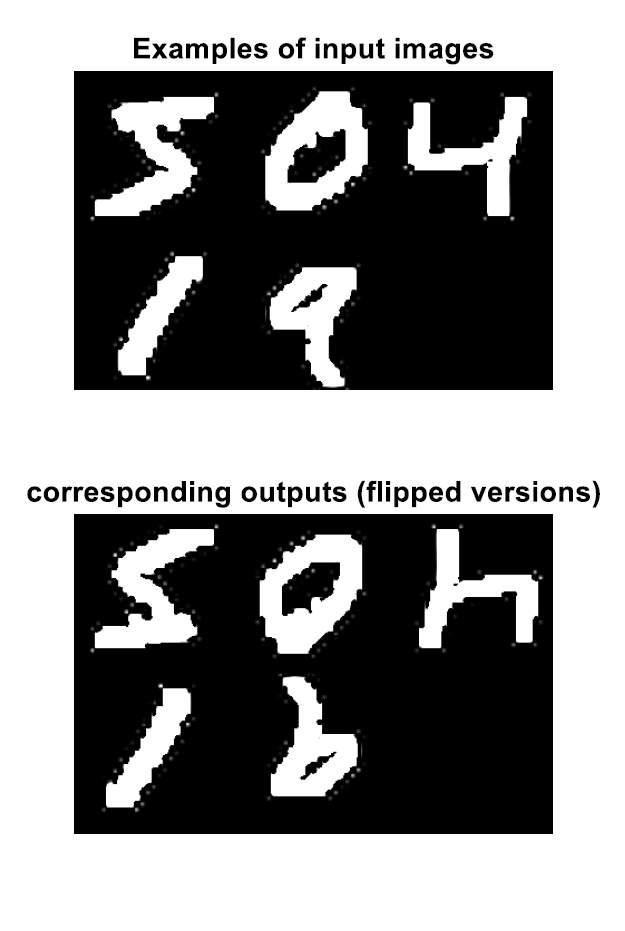
\includegraphics[width=0.5\textwidth]{example_outputs.png}}}
			\label{example_outputs}
		\end{figure}
		
		Note: You can use any programming language and libraries for this problem. Please submit your code with the homework so that the graders can run it if needed.

		\begin{enumerate}
			\item[1)] Implement and train the network so that when an image from the MNIST set is presented, the output is its flipped version. Show the learning curve and the final MSE value achieved on the training set.
			
			\begin{figure}[H]
				\centerline{\fbox{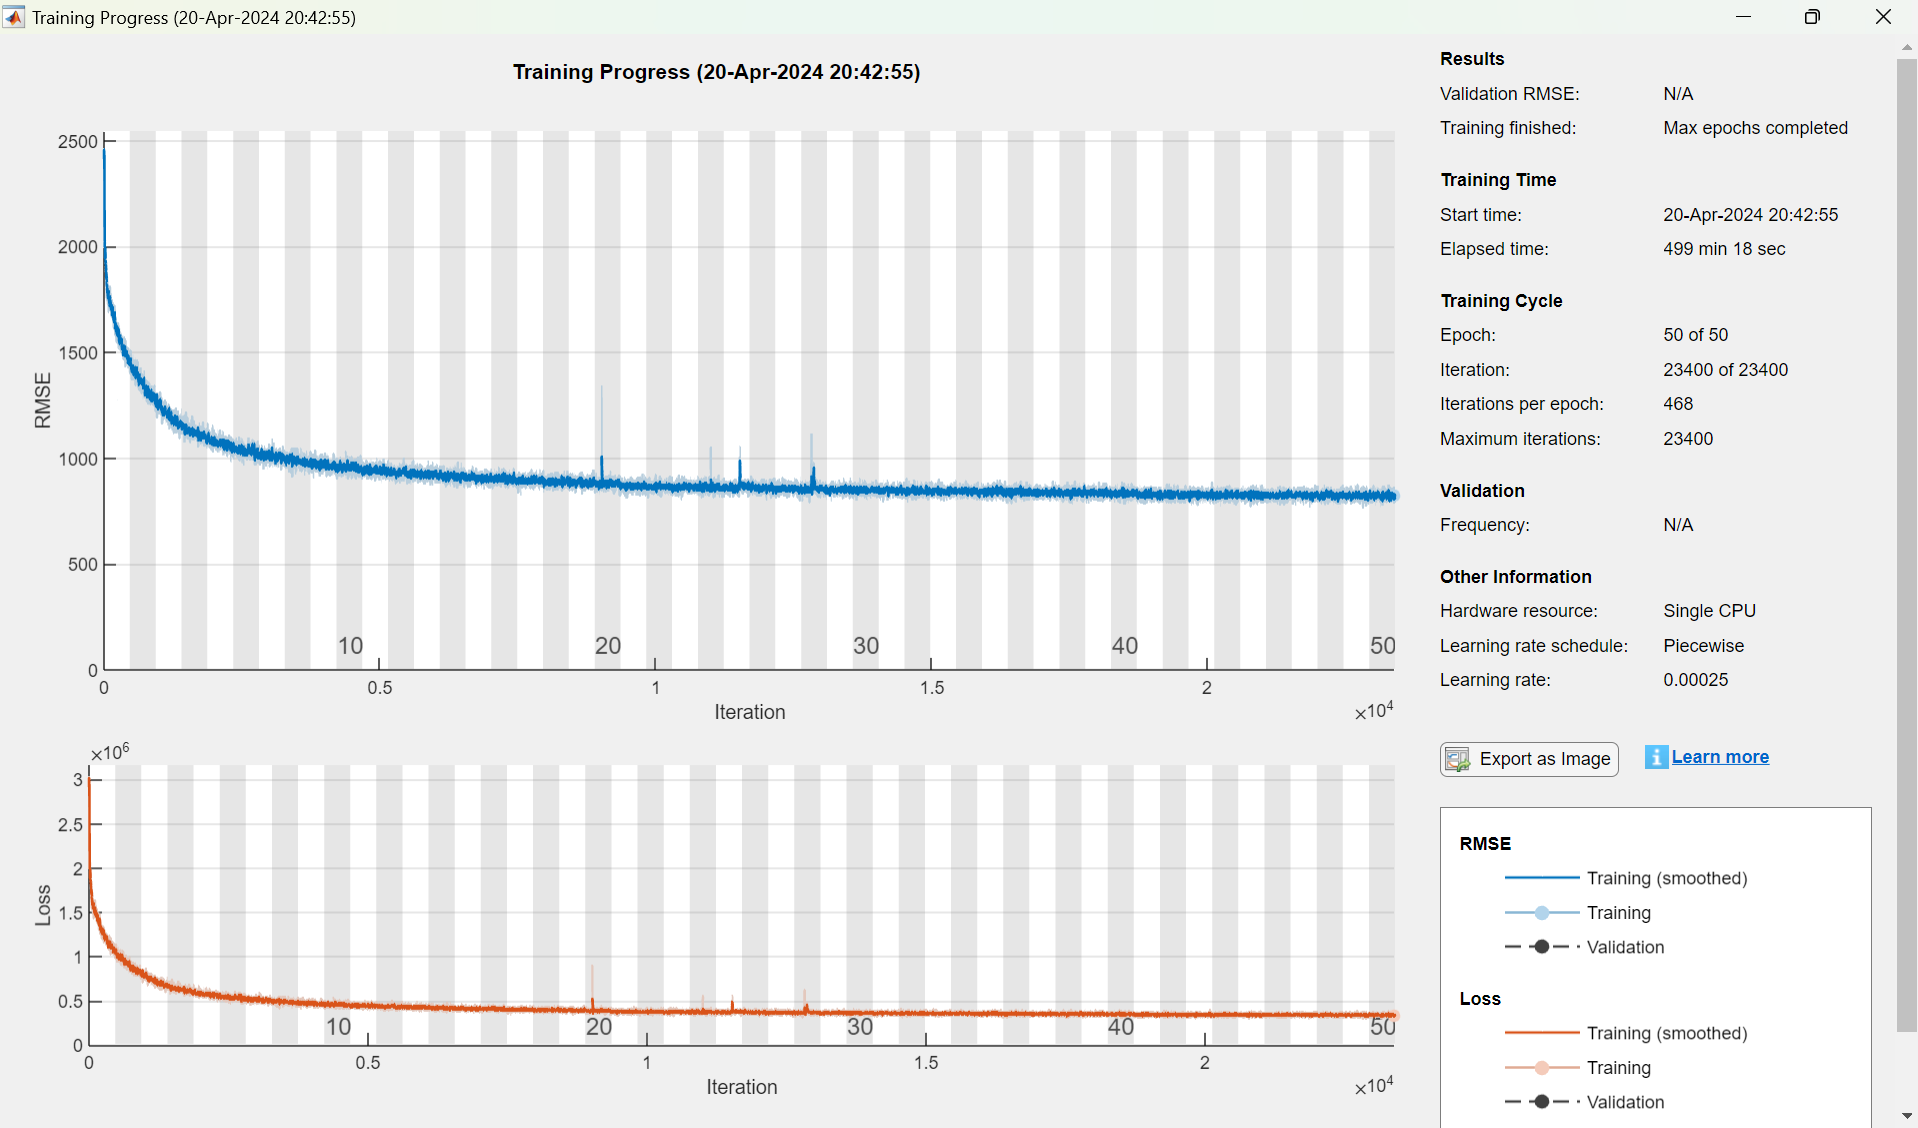
\includegraphics[width=0.9\textwidth]{learning_curve.png}}}
				\caption{Learning Curve}
				\label{learning_curve}
			\end{figure}
			
			\begin{figure}[H]
				\centerline{\fbox{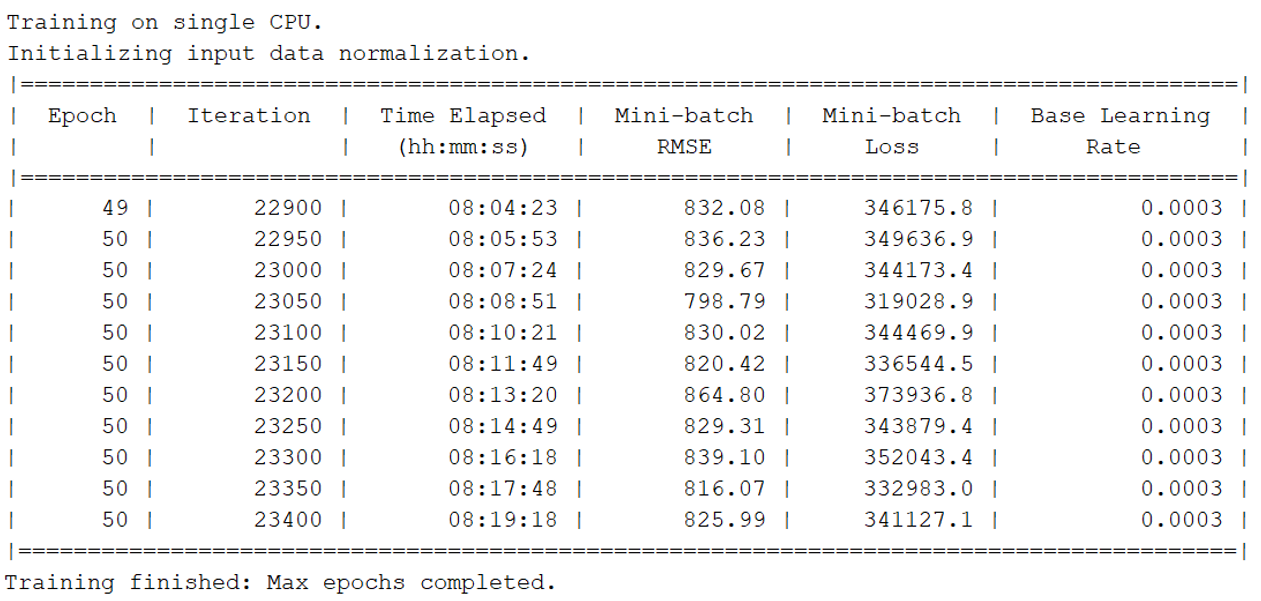
\includegraphics[width=0.9\textwidth]{combined_printout.png}}}
				\caption{Training Printout}
				\label{training_printout}
			\end{figure}
			
			\begin{figure}[H]
				\centerline{\fbox{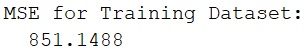
\includegraphics[width=0.4\textwidth]{mse_training.png}}}
				\caption{MSE for Training Dataset}
				\label{training_mse}
			\end{figure}
			
			\pagebreak
			\item[2)] Show examples of the results on each digit from 0 to 9 using both the training and test sets.
			
			\begin{figure}[H]
				\centerline{\fbox{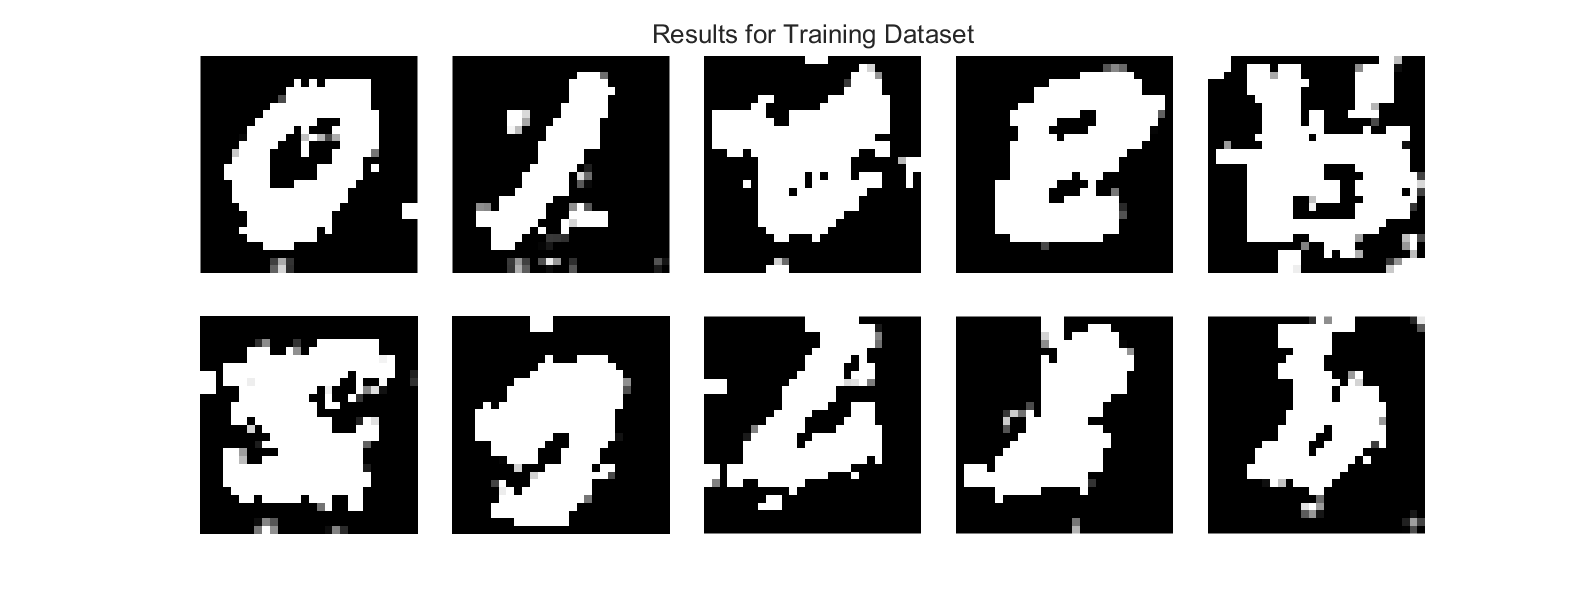
\includegraphics[width=0.9\textwidth]{training_results.png}}}
				\caption{Results for Training Set}
				\label{training_results}
			\end{figure}
			
			\begin{figure}[H]
				\centerline{\fbox{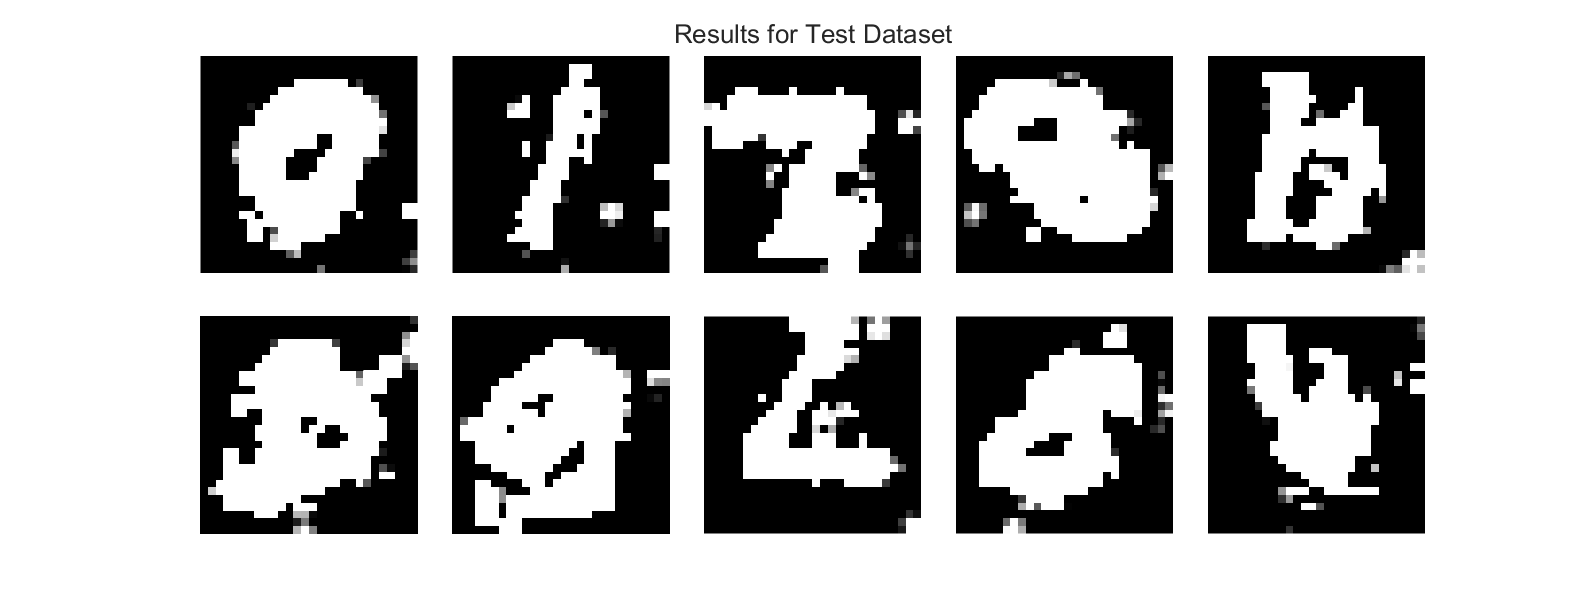
\includegraphics[width=0.9\textwidth]{test_results.png}}}
				\caption{Results for Test Set}
				\label{test_results}
			\end{figure}
			
			\item[3)] Which digit achieves the lowest MSE on the training and tests sets? Are they the same?
			
			\begin{figure}[H]
				\centerline{\fbox{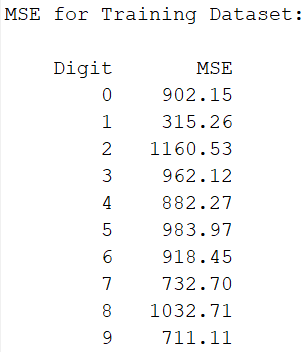
\includegraphics[width=0.4\textwidth]{mse_per_digit_training.png}}}
				\caption{Per Digit MSE for Training Set}
				\label{mse_per_digit_training}
			\end{figure}
			
			\begin{figure}[H]
				\centerline{\fbox{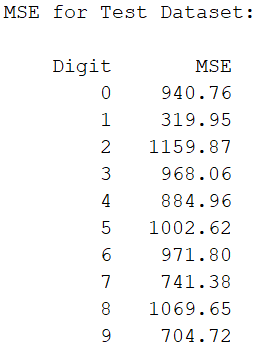
\includegraphics[width=0.35\textwidth]{mse_per_digit_test.png}}}
				\caption{Per Digit MSE for Test Set}
				\label{mse_per_digit_test}
			\end{figure}
			
			The digit 1 achieves the lowest MSE for both the training and test sets. For the training set it has an MSE 315.26, and for the test set, it has an MSE of 319.65.
			
			\item[4)] The dimensions of the embedded space are 5 x 5 x 16. Obtain the activations for this layer using all the training images and flatten each of them into vectors of length 400. Show the histograms of the first five features.
			
			\begin{figure}[H]
				\centerline{\fbox{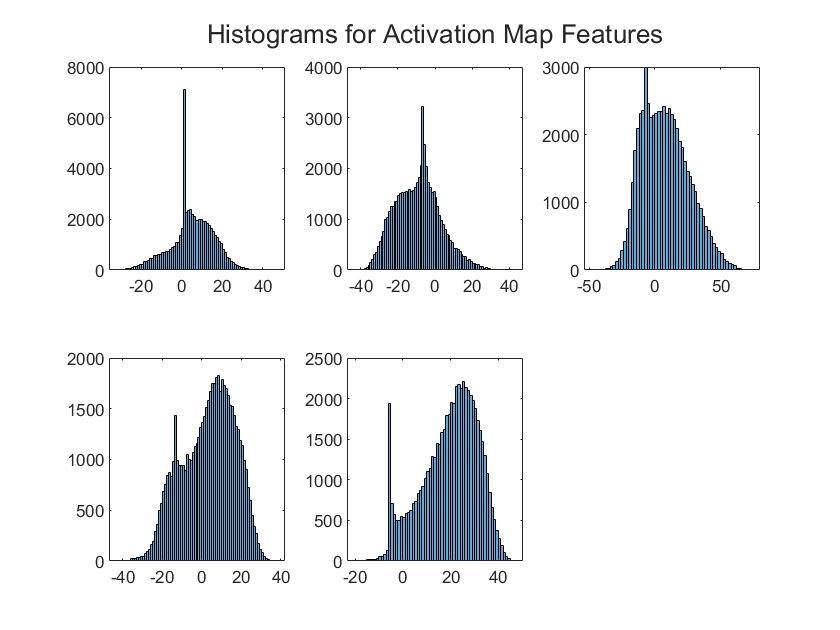
\includegraphics[width=0.8\textwidth]{activation_map_histogram.png}}}
				\caption{Histograms of First Five Activation Features}
				\label{acivation_histograms}
			\end{figure}
			
			\pagebreak
			\item[5)] Comment on the shape of the distributions. What are the mean and variance of the first five features? Calculate the covariance matrix for these features, and generate a set five-dimensional gaussian
random vector using this covariance matrix and mean values. Compare the histograms of the data you generate to the ones of the features obtained from the training images and comment on how well they seem
to match.

			The shape of the measured distributions roughly mirror Gaussian distributions.
			
			\begin{figure}[H]
				\centerline{\fbox{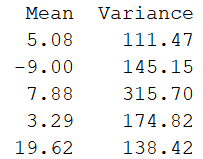
\includegraphics[width=0.3\textwidth]{mean_and_variance.png}}}
				\caption{Mean and Variance of First Five Activation Features}
				\label{mean_and_var}
			\end{figure}
			
			\begin{figure}[H]
				\centerline{\fbox{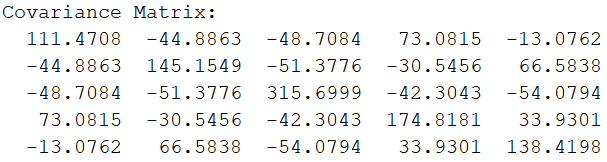
\includegraphics[width=0.85\textwidth]{covariance_matrix.png}}}
				\caption{Covariance Matrix}
				\label{covariance_matrix}
			\end{figure}
			
			\begin{figure}[H]
				\centerline{\fbox{\includegraphics[width=0.8\textwidth]{generated_data_histogram.png}}}
				\caption{Histograms of Generated Data}
				\label{generated_data_histogram}
			\end{figure}
			
			The histograms of the measured data are slightly skewed and contain tight clusters of data. This is not replicated in the histograms of the generated data. However, the resulting histograms still roughly approximate those of the measured data.	
		\end{enumerate}
	\end{enumerate}
	
	\pagebreak
	\appendix
	\section{Source Code}
	\label{source_code}
	\lstset{style=Matlab-editor,basicstyle=\ttfamily\footnotesize}
	\lstinputlisting{Homework6_Sowatzke.m}
	\lstinputlisting{loadMNISTData.m}
	\lstinputlisting{readBinaryFile.m}
	\raggedbottom
\end{document}